\section{Completación simultánea en una reserva espectral}\label{sec:spectral-reserve}

Primero usamos las reservas ponderadas de Hall para emparejar a los excepcionales libres de cada color. Luego emparejamos los ordinarios que quedan libres mediante dos conjuntos disjuntos de copias cruzadas. Uno da emparejamientos parciales para toda la paleta. El otro da recorridos que reparan esos emparejamientos sin volver a usar una copia.

\subsection{El lema de reparación}

En un bloque ordinario, los dos lados físicos tienen tamaño \(N\). Para cada color \(i\), los conjuntos libres de ambos lados tienen igual tamaño y \(M_i\) es un emparejamiento inicial entre ellos. Escribimos \(X_i,Y_i\) para los vértices libres que \(M_i\) deja sin cubrir, y \(A_i^-,B_i^-\) para todos los vértices físicos que \(M_i\) deja sin cubrir. Estos últimos conjuntos incluyen los vértices no disponibles en el color.

\begin{lemma}[Reparación en una reserva espectral]\label{lem:spectral-repair}
Sea \(R\) un grafo bipartito simple \(d\)-regular sobre los dos lados físicos, con \(d>0\). Cada arista de \(R\) representa una copia cruzada reservada para reparaciones. Los emparejamientos iniciales usan copias fuera de \(R\) y son disjuntos dos a dos en copias. Supongamos que la matriz de biadyacencia normalizada \(P\) de \(R\) tiene norma de operador a lo sumo \(\sigma<1\) en los vectores de media cero. Sea \(h\ge1\) tal que \(\sigma^h\le1/(2N)\) y pongamos \(\ell=2h+1\).

En cada color, cada vértice físico tiene a lo sumo \(\rho d\) vecinos de reserva en el conjunto opuesto \(A_i^-\) o \(B_i^-\) que quedó sin cubrir. Cada vértice físico pertenece a lo sumo a \(t\) de los conjuntos libres que quedaron sin cubrir en su propio lado. Si hay \(k\) colores y
\[
 3(\ell-1)\rho\le\frac12,\qquad
 6\ell\,\frac{2t+(\ell-2)k\rho}{d}+6(\ell-1)^2\rho\le\frac{4}{27},
 \tag{P}\label{eq:spectral-repair}
\]
entonces se pueden emparejar todos los conjuntos ordinarios libres usando copias cruzadas disjuntas dos a dos de los emparejamientos iniciales y de \(R\).
\end{lemma}

\begin{proof}
Para cada color extendemos \(M_i\) a una biyección \(\pi_i\) del lado físico izquierdo al derecho, emparejando \(X_i\) con \(Y_i\) y emparejando por separado los vértices no disponibles. Cada par \(x,\pi_i(x)\) con \(x\in X_i\) es una solicitud. Identificamos los estados derechos con las coordenadas izquierdas mediante \(\pi_i^{-1}\). La matriz de transición sobre esas coordenadas es \(K_i(u,v)=P(u,\pi_i(v))\). Un recorrido para la solicitud \(x\) empieza en \(x\), da \(\ell\) pasos de reserva y está condicionado a terminar en la coordenada \(x\).

Tanto \(K_i\) como \(K_i^{\mathsf T}\) conservan las constantes y contraen los vectores de media cero por un factor a lo sumo \(\sigma\). Una masa puntual centrada tiene norma euclidiana a lo sumo uno, así que cada entrada para un tramo de al menos \(h\) pasos difiere de \(1/N\) en a lo sumo \(\sigma^h\). Por consiguiente, cada entrada está entre \(1/(2N)\) y \(3/(2N)\). Invertir la lista de estados y sustituir \(K_i\) por \(K_i^{\mathsf T}\) conserva el producto de las probabilidades de transición y la masa en los extremos que lo normaliza. Así se obtiene la misma ley condicionada a los extremos al leer el recorrido al revés. En cualquier paso de reserva, el tramo estrictamente anterior o el estrictamente posterior tiene longitud al menos \(h\). Al leer desde el extremo con el tramo más corto, todo evento determinado hasta el paso elegido aumenta su probabilidad por un factor a lo sumo \(3\) al condicionar por los extremos. Esto se sigue de dividir la cota superior \(3/(2N)\) para el tramo no examinado por la cota inferior \(1/(2N)\) para la masa en los extremos.

Una coordenada intermedia es admisible cuando representa un par de \(M_i\). En cada posición intermedia, uno de los dos tramos adyacentes tiene longitud al menos \(h\). Antes de condicionar, un paso hacia esa posición llega a una coordenada prohibida con probabilidad a lo sumo \(\rho\), por la cota de vecinos de reserva en \(B_i^-\) en el recorrido directo o en \(A_i^-\) en el inverso. El condicionamiento por los extremos eleva la cota a \(3\rho\). La primera desigualdad de \eqref{eq:spectral-repair} y la cota de la unión dan probabilidad condicional al menos \(1/2\) de que todas las coordenadas intermedias sean admisibles. Restringirnos a esos recorridos aumenta las cotas siguientes por un factor adicional de a lo sumo dos.

Para contar cuánto puede usarse una copia de reserva, iniciamos un recorrido sin condicionar desde cada \(x\in X_i\). Después del primer paso, la masa total en cada coordenada es a lo sumo \(\rho\), pues a lo sumo \(\rho d\) vecinos de \(A_i^-\) pueden enviarle masa \(1/d\). La matriz de transición conserva esa cota superior porque sus columnas suman uno. Los recorridos inversos respetan la misma cota al partir de \(Y_i\). En un paso interior de reserva tomamos la dirección con el tramo largo sin examinar. La masa total que atraviesa una copia fija en ese paso y color es a lo sumo \(\rho/d\) antes de condicionar. Después de ambos condicionamientos es a lo sumo \(6\rho/d\). En un paso extremo, solo las solicitudes que empiezan o terminan en el vértice físico correspondiente pueden usar la copia, así que la cota en toda la paleta es \(6t/d\) en cada extremo. Para una arista del emparejamiento anterior contamos solo solicitudes de su color. En cada posición intermedia la cota superior es \(6\rho\), por el mismo argumento con la masa en la coordenada contraída. Sumando sobre las posiciones se acotan las probabilidades de usar un recurso al menos una vez, sumadas sobre todas las solicitudes,
\[
 \mu_R=\frac{6\bigl(2t+(\ell-2)k\rho\bigr)}{d}
 \qquad\text{y}\qquad
 \mu_M=6(\ell-1)\rho.
\]

Elegimos los recorridos independientemente, uno por solicitud. Para dos solicitudes distintas \(p,q\), el evento \(E_{pq}\) es que compartan una copia de reserva o una arista del emparejamiento anterior de su color común. Una cota de la unión sobre los recursos del recorrido de \(p\), seguida de un promedio sobre ese recorrido, da
\[
 \sum_{q\ne p}\Pr(E_{pq})\le\ell\mu_R+(\ell-1)\mu_M\le\frac{4}{27}.
\]
En el grafo de dependencias, dos eventos son adyacentes cuando se intersecan sus pares de solicitudes. Un evento es independiente de toda la colección de eventos cuyos pares evitan el suyo, pues las elecciones de base son independientes. Para un evento \(E_{pq}\) de probabilidad positiva ponemos \(x_{pq}=\tfrac94\Pr(E_{pq})\le1/3\). Dividimos sus vecinos en los que involucran a \(p\) y los restantes, que involucran a \(q\). En cada grupo la suma de los \(x\) es a lo sumo \(\tfrac94\cdot\tfrac4{27}=\tfrac13\). Cada grupo aporta un producto de \(1-x\) de al menos \(2/3\) por la cota \(\prod_j(1-x_j)\ge1-\sum_j x_j\). El producto sobre ambos grupos es al menos \(4/9\), y \(x_{pq}\cdot4/9=\Pr(E_{pq})\). El lema local asimétrico de Lovász~\cite{EL} da una elección de recorridos que evita todos los conflictos.

Para un color fijo, consideremos el grafo de aristas utilizables formado por su emparejamiento anterior y las copias de reserva de sus recorridos elegidos. Verificamos la desigualdad de Hall en las coordenadas contraídas. Para un conjunto \(S\) de coordenadas libres izquierdas, el emparejamiento anterior da los vecinos derechos \(S\setminus X_i\). Una solicitud en \(x\in S\cap X_i\) recorre desde \(x\) hasta \(x\). Su primer paso de reserva con llegada fuera de \(S\setminus X_i\) sale de \(S\). La llegada es su propio extremo sin emparejar o una coordenada emparejada. Estas llegadas son distintas para solicitudes distintas, pues los extremos sin emparejar se asignaron mediante una biyección y compartir una coordenada emparejada reutilizaría una arista del emparejamiento anterior. Así hay \(|S\cap X_i|\) vecinos derechos adicionales. Esto prueba la desigualdad de Hall para todo \(S\). Los emparejamientos resultantes solo usan las copias asignadas a sus respectivos colores. Dos colores pueden pasar por el mismo vértice físico, como en la Figura~\ref{fig:repair}.
\end{proof}

\begin{figure}[htbp]
\centering
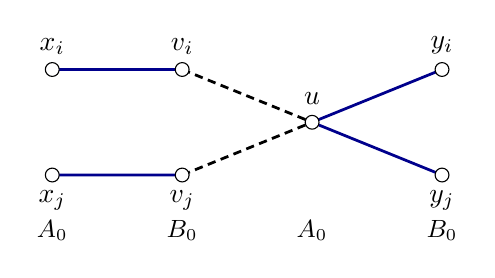
\begin{tikzpicture}[x=1.65cm,y=.67cm,
  vertex/.style={circle,draw,fill=white,inner sep=1.3pt,minimum size=5pt},
  reserve/.style={line width=1pt,blue!55!black},
  matched/.style={line width=1pt,densely dashed}]
  \coordinate (xi) at (0,1); \coordinate (xj) at (0,-1);
  \coordinate (vi) at (1,1); \coordinate (vj) at (1,-1);
  \coordinate (u) at (2,0);
  \coordinate (yi) at (3,1); \coordinate (yj) at (3,-1);
  \draw[reserve] (xi)--(vi) (xj)--(vj) (u)--(yi) (u)--(yj);
  \draw[matched] (vi)--(u) (vj)--(u);
  \foreach \name in {xi,xj,vi,vj,u,yi,yj} \node[vertex] at (\name) {};
  \foreach \name/\lab in {xi/x_i,vi/v_i,yi/y_i}
     \node[above=2pt] at (\name) {$\lab$};
  \foreach \name/\lab in {xj/x_j,vj/v_j,yj/y_j}
     \node[below=2pt] at (\name) {$\lab$};
  \node[above=3pt] at (u) {$u$};
  \foreach \col/\side in {0/$A_0$,1/$B_0$,2/$A_0$,3/$B_0$}
     \node[font=\small] at (\col,-2.05) {\side};
\end{tikzpicture}
\caption{Dos colores pueden pasar por el mismo vértice izquierdo \(u\). En el color \(i\), la arista discontinua \(v_i u\) pertenece al emparejamiento anterior y las dos aristas continuas son copias de reserva. El recorrido de abajo repara el color \(j\) con otras copias de reserva. Dentro de un color, un segundo recorrido por el mismo vértice emparejado reutilizaría su arista del emparejamiento anterior.}\label{fig:repair}
\end{figure}

\subsection{Un criterio de factorización mediante un \emph{nibble}}

Supongamos que los dos lados físicos de ordinarios tienen tamaño \(N\). Sea \(C\) un conjunto de copias cruzadas ordinarias disjunto de la reserva \(R\). Dados los conjuntos ordinarios libres \(F_i,G_i\), el hipergrafo de incidencia tiene un vértice por cada demanda izquierda \((i,x)\) con \(x\in F_i\), uno por cada demanda derecha \((i,y)\) con \(y\in G_i\) y uno por cada copia \(e\in C\). Cada uso elegible de una copia \(e=xy\) da la terna
\[
 \{(i,x),(i,y),e\}.
\]
La elegibilidad requiere \(x\in F_i\) e \(y\in G_i\). El grado de una demanda cuenta copias elegibles. El grado de una copia cuenta colores elegibles. Un cogrado puede exceder uno solo para dos demandas de lados opuestos en el mismo color, cuando hay copias paralelas elegibles entre sus extremos.

Usamos la estimación del \emph{nibble} de Keevash~\cite[Sección~3.1]{KeevashII}, en la forma de pesos iguales que se deriva de Ehard, Glock y Joos~\cite{EGJ}. Fijemos \(0<\delta<1\). Para \(\Delta\) suficientemente grande en función de \(\delta\), sea el hipergrafo de incidencia de grado máximo a lo sumo \(\Delta\), cogrados a lo sumo \(\Delta^{1-\delta}\) y todos los grados de demanda al menos \((1-\eta)\Delta\), donde \(0\le\eta<1\). Si el número de ternas y el número de pruebas son cada uno a lo sumo \(\exp(\Delta^{(\delta/450)^2})\), existe un emparejamiento que deja masa sin cubrir a lo sumo
\[
 B(z)=\max\left\{(\eta+\Delta^{-\delta/450})z,\frac{3\Delta^\delta}{1-\eta}\right\}
 \label{eq:nibble-error}\tag{N}
\]
en cada prueba elegida con soporte en las demandas, pesos en \([0,1]\) y masa total \(z\).

\begin{theorem}[Factorización a partir de reservas ponderadas y un \emph{nibble}]\label{thm:hybrid-completion}
Fijemos \(0<\delta<1\). Sea \(M\) un multigrafo \(D\)-regular con un corte equilibrado e igual número de ordinarios a cada lado. Sus aristas internas tienen un coloreo propio con \(k\le D\) colores, que deja el mismo número de vértices libres en los dos lados para cada color.

Designemos copias cruzadas separadas para las filas excepcionales en ambas orientaciones, un conjunto ordinario \(C\) y una reserva ordinaria simple \(d\)-regular \(R\), con \(d>0\). En cada par, la suma de copias designadas es a lo sumo su multiplicidad en \(M\). Las dos orientaciones de filas excepcionales tienen los siguientes certificados ponderados de Hall. Para una fila \(x\), sea \(\eta_x\ge0\) su costo por copia gastada. Su peso en una columna ordinaria está entre cero y \(\eta_x\) por la multiplicidad designada en ese par. El peso total de una columna es a lo sumo una cota positiva común. En cada color, una fila excepcional libre tiene en las columnas ordinarias libres peso al menos esa cota más \((k-1)\eta_x\). Las estimaciones suficientes \eqref{eq:rowx} y \eqref{eq:rowy} dan estos certificados al medirlas sobre las copias designadas.

Supongamos que después de cualquier elección factible de emparejamientos entre excepcionales y ordinarios que cubra todos los excepcionales libres y respete las copias designadas, se cumplen las siguientes condiciones sobre los conjuntos ordinarios libres \(F_i,G_i\) restantes.
\begin{enumerate}
\item Para algún \(\Delta\) suficientemente grande en función de \(\delta\) y algún \(0\le\eta<1\), el hipergrafo de incidencia de \(C\) satisface las cotas de grado y cogrado de \eqref{eq:nibble-error}. Tanto su número de ternas como \(2N(k+1)\) son a lo sumo \(\exp(\Delta^{(\delta/450)^2})\).
\item La matriz normalizada de \(R\) tiene norma a lo sumo \(\sigma<1\) sobre vectores de media cero. Cada vértice físico tiene a lo sumo \(\beta d\) vecinos de reserva fuera del conjunto libre opuesto de cualquier color. Para un entero \(h\ge1\) con \(\sigma^h\le1/(2N)\), las cantidades
\[
 \ell=2h+1,\qquad t=B(k),\qquad \rho=\beta+B(d)/d
\]
satisfacen \eqref{eq:spectral-repair}.
\end{enumerate}
Entonces los \(k\) colores internos se extienden a emparejamientos perfectos con copias cruzadas disjuntas dos a dos y \(M\) tiene una 1-factorización.
\end{theorem}

\begin{proof}
El argumento ponderado de Hall del Teorema~\ref{thm:factor} cubre los vértices excepcionales. En cada orientación, los a lo sumo \(k-1\) colores anteriores pueden reducir el peso de una fila en a lo sumo \((k-1)\eta_x\). Las cotas restantes de filas y columnas dan la desigualdad de Hall. Las dos orientaciones cubren conjuntos disjuntos de vértices en cada color, pues cada una une un excepcional con un ordinario. Retiran el mismo número de vértices en cada lado del corte, por lo que \(|F_i|=|G_i|\).

Usamos dos clases de pruebas con indicadores en el \emph{nibble}. En cada vértice físico contamos sus demandas a lo largo de la paleta, a lo sumo \(k\). Para cada color y vértice físico contamos las demandas libres opuestas entre sus vecinos de reserva, a lo sumo \(d\). Hay \(2N(k+1)\) pruebas. El emparejamiento de ternas da emparejamientos iniciales \(M_i\) en \(C\) con copias físicas distintas en todos los colores. Las primeras pruebas acotan por \(B(k)\) el número de conjuntos libres sin cubrir que contienen a cualquier vértice. Las segundas acotan por \(B(d)\) el número de vecinos ordinarios que quedan sin cubrir en cada vértice y color. Al añadir los vecinos ya no disponibles resulta la cota \(\beta d+B(d)=\rho d\) para los conjuntos sin cubrir del Lema~\ref{lem:spectral-repair}.

El lema completa los emparejamientos ordinarios. Sus copias y las que usaron los emparejamientos de excepcionales respetan las capacidades designadas en cada par físico. Junto con las aristas internas dan \(k\) emparejamientos perfectos disjuntos. El residuo tiene grado \(D-k\) y contiene solo copias cruzadas, por lo que se factoriza por el teorema de Hall.
\end{proof}

El teorema de Hall da los emparejamientos de excepcionales a partir de las cotas de filas y columnas. Los grados de demanda ordinarios y las vecindades de reserva dependen de los vértices que usen esos emparejamientos. Una cota de pérdidas válida para cada emparejamiento factible permite aplicar las estimaciones ordinarias a la elección que da Hall. Si cada lado pierde a lo sumo \(s\) ordinarios, cada vértice de un conjunto simple de copias pierde a lo sumo \(s\) vecinos en el lado opuesto. Eliminar ternas elegibles conserva las cotas superiores de grados de copia y cogrados. Usamos estas cotas en la rejilla que sigue.

\subsection{Una familia dispersa de rejillas fuera del criterio de rectángulos}\label{sec:sparse-reserve-example}

Fijemos enteros \(b\ge1\) y \(q\ge12\) par. Cada lado tiene \(N=bq^2\) ordinarios en una rejilla de \(q\) por \(q\) con \(b\) vértices por celda. Numeramos filas y columnas de \(0\) a \(q-1\). Dos vértices opuestos son adyacentes en el soporte de la rejilla cuando comparten fila o columna. Cada par del soporte tiene una copia en \(C\) y otra en \(R\), de modo que ambos conjuntos tienen grado \(d=b(2q-1)\). Sobre vectores constantes en cada celda, la matriz del soporte es \(b(J_q\otimes I_q+I_q\otimes J_q-I_{q^2})\), donde \(J_q\) es la matriz de unos. El valor propio sobre las constantes es \(d\). Si exactamente una de las funciones de coordenada tiene suma cero, el valor propio es \(b(q-1)\). Si ambas tienen suma cero, es \(-b\). En vectores de suma cero en cada celda, la matriz es cero. Por tanto, la norma de la reserva normalizada sobre el espacio de media cero es \((q-1)/(2q-1)<1/2\).

Ponemos \(d\) copias en un par interno izquierdo y en uno derecho. Los pares usan las columnas \(0,1\) en la fila \(0\) de la izquierda y en la fila \(q/2\) de la derecha. Una copia de cada par va en cada uno de \(k=d\) colores. Los ordinarios internamente libres se emparejan a través del corte por coordenadas iguales donde es posible. Las dos coordenadas izquierdas restantes en la fila \(q/2\) se emparejan con las dos derechas restantes en la fila \(0\) en sus columnas respectivas. Cada par de esta biyección recibe \(d\) copias de relleno.

Hay \(r=\lfloor\sqrt q\rfloor\) excepcionales por lado, emparejados a través del corte. Para cada par excepcional \(x,y\) elegimos dos pares de relleno \(u_L,u_R\) de coordenadas iguales en la fila \(q/2+1\), con las \(2r\) coordenadas distintas entre los excepcionales. Esto es posible pues \(2r\le q\). En cada coordenada elegida, las \(d\) copias de relleno se sustituyen por \(d\) de \(u_Ly\) y \(d\) de \(xu_R\). Ponemos también \(d\) copias en \(xy\). Las sustituciones conservan cada grado ordinario, que es \(3d\) por los dos conjuntos de la rejilla y las copias internas o de relleno. Un excepcional tiene dos vecinos ordinarios de multiplicidad \(d\) y su pareja excepcional de multiplicidad \(d\), así que también tiene grado \(3d\).

\paragraph{Los parámetros del criterio híbrido.}
Cada fila excepcional puede dar peso \(d\) a sus dos vecinos ordinarios, con la misma cota de columna y costo uno. Esos vecinos están inicialmente libres en todos los colores y cada columna pertenece a una sola fila en cada orientación. Después de cualquier emparejamiento factible de los excepcionales, cada lado ordinario libre tiene tamaño \(N-r-2\). Un vértice físico pierde a lo sumo \(r+2\) vecinos en cada conjunto de la rejilla. El hipergrafo de incidencia tiene entonces grado máximo a lo sumo \(d\), cogrado a lo sumo uno y grados de demanda al menos \(d-r-2\). El número de ternas es a lo sumo \(kNd\) y el de pruebas es \(2N(k+1)\), ambos polinomiales en \(q\).

Tomamos \(\Delta=k=d\), \(\delta=1/4\) y \(\eta=\beta=(r+2)/d\). Con \(b\) fijo, \(\eta=O(d^{-1/2})\) y
\[
 \frac{B(d)}{d}
 =\max\left\{\eta+d^{-1/1800},\,\frac{3d^{-3/4}}{1-\eta}\right\}
 =O(d^{-1/1800}).
\]
Así, tanto \(t/d\) como \(\rho\) son \(O(d^{-1/1800})\). Tomando \(h=\lceil\log_2(2N)\rceil\) se obtiene \(\ell=O(\log N)\). Como \(k=d\), ambos lados izquierdos de \eqref{eq:spectral-repair} están acotados por \(O((\log N)^2d^{-1/1800})=o(1)\). Esto da la aplicación asintótica del Teorema~\ref{thm:hybrid-completion}.

\begin{corollary}[Factorización de la rejilla y separación del criterio de rectángulos]\label{cor:sparse-grid}
Para todo \(b\ge1\) y \(q\ge12\) par, el multigrafo recién construido tiene una 1-factorización. Tiene \(d=\Theta(\sqrt N)\) vecinos ordinarios cruzados distintos por vértice ordinario y \(r=\Theta(N^{1/4})\) excepcionales por lado para \(b\) fijo. El criterio de rectángulos del Teorema~\ref{thm:factor} falla para toda paleta interna admisible en este corte.
\end{corollary}

\begin{proof}
El umbral explícito proviene de los pares de relleno. En cada una de las \(d\) rondas usamos una copia de cada arista interna. En la primera coordenada modificada para \(x,y\), emparejamos \(u_L\) con \(y\) y \(x\) con \(u_R\), usando copias nuevas en cada ronda. La segunda coordenada modificada para cada par de excepcionales queda sin cubrir en ambos lados. La llamamos un hueco. Un hueco puede intercambiar su relleno ausente con cualquier vecino de la rejilla cuyo relleno diagonal sigue intacto. Al excluir las cuatro coordenadas de extremos internos y las \(2r\) coordenadas modificadas quedan al menos \(d-(2r+4)\) opciones en cada hueco.

Mostramos que los intercambios se pueden programar siempre que
\[
 r\le m_0=\left\lceil\frac d2\right\rceil
 \qquad\text{y}\qquad
 \left\lfloor\frac d2\right\rfloor\ge 2r+4.
\]
Cada hueco tiene entonces al menos \(m_0\) ayudantes elegibles. Elegimos exactamente \(m_0\) para cada hueco. Así obtenemos un grafo bipartito simple de grado \(m_0\) en cada hueco y a lo sumo \(r\le m_0\) en cada ayudante. Por el teorema de coloreo bipartito de aristas de K\H{o}nig, estos pares se dividen en \(m_0\) emparejamientos. Cada uno cubre todos los huecos y los ayudantes usados en una ronda son distintos. Para \(q\ge12\), tenemos \(q\ge2r+5\). Si \(r\le3\), esto se sigue de \(q\ge12\), y si \(r\ge4\), de \(q\ge r^2\). Como \(\lfloor d/2\rfloor\ge q-1\), ambas desigualdades valen para todo \(b\ge1\).

Duplicamos la programación, asignamos las dos ocurrencias a conjuntos distintos de copias de la rejilla y conservamos \(d\) de las \(2m_0\) rondas. Si un hueco en la coordenada \(z\) usa un ayudante en \(w\), su intercambio usa \(z_Lw_R\) y \(w_Lz_R\). Ambos pares existen porque compartir fila o columna es simétrico. Los intercambios de una ronda son disjuntos. El conjunto y los extremos de una copia identifican su hueco, su ayudante y su dirección. Cada hueco usa un ayudante dado a lo sumo una vez en cada conjunto, así que todas las copias de los intercambios son distintas. Los ayudantes no usados y los dos pares de relleno fuera de la diagonal usan copias separadas de sus rellenos en cada ronda. Esto da \(d\) emparejamientos perfectos disjuntos que contienen las copias internas. El residuo es \(2d\)-regular y bipartito, de modo que se factoriza.

Para la separación, sea \(S\) la primera mitad izquierda de las filas y \(T\) la segunda mitad derecha. Sus tamaños suman \(N\). En ambas direcciones, cada vértice de este rectángulo ve \(bq/2\) vértices de la otra mitad a través de su columna y usa dos copias de la rejilla para cada uno. Las copias de relleno en coordenadas iguales y los dos rellenos de la segunda mitad izquierda a la primera mitad derecha aportan cero al rectángulo. Así, todo vértice tiene \(bq<d\) copias al conjunto opuesto. Un coloreo interno propio requiere al menos \(d\) colores porque cada par interno tiene \(d\) copias paralelas. El rectángulo excede el umbral \(N-r-2a\) del Teorema~\ref{thm:factor}, y las copias por vértice son menos que el tamaño de cualquier paleta admisible. El soporte cruzado ordinario es exactamente el de la rejilla, pues los rellenos fuera de la diagonal comparten columna. Con \(b\) fijo, las expresiones de \(N,d,r\) dan los órdenes de crecimiento indicados.
\end{proof}

La rejilla separa el criterio de rectángulos de la factorización en el corte dado. El umbral explícito \(q\ge12\) usa el emparejamiento de relleno para programar intercambios deterministas. El Teorema~\ref{thm:hybrid-completion} usa los conjuntos de copias ordinarias y de reserva bajo sus hipótesis de grado y espectrales, que se cumplen para esta rejilla para todo \(q\) suficientemente grande con \(b\) fijo.
